\newpage
\section{De Moivre Saves the Day!}

The rules for solving second and third degree equations led to a
``sticky wicket.''  Namely the rule for solving a quadratic equation
forced its user to take the square root of a number that was sometimes
negative.  Worse yet, the formula for solving a cubic equation forced
the user to take the cube root of a number that resulted from taking
square roots!  Despite misgivings, mathematicians were eventually
forced to expand the number system to one where square roots can be
found for any of its numbers.

You may recall that the Ferro-Tartaglia method gives 
\[
\sqrt[3]{\frac{-1+\sqrt{-31}}{2}} + \frac{2}{\sqrt[3]{\frac{1}{2}(-1+\sqrt{-31})}}
\]
as a solution to: $y = x^3-6x+1$. Moreover, as this plot of $y = x^3-6x+1$ shows
\[
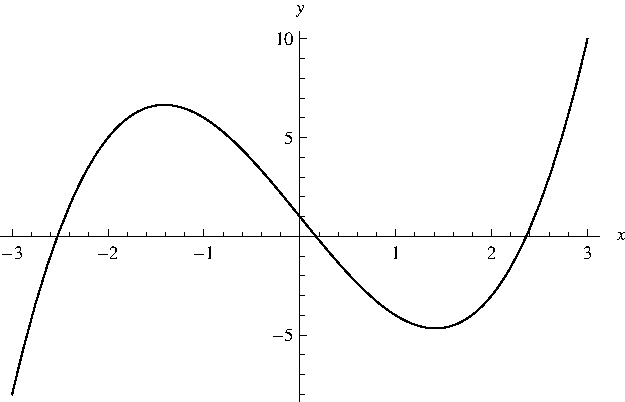
\includegraphics[width=3in]{../graphics/cubicPlot.pdf}
\]
this must be a real solution\dots But how? There is a square-root of a
negative number in the expression above! 

We're going to investiagate incredible connection between adding and
multiplying complex numbers and plane geometry.  It's called \textit{De
Moivre's rule}---it is here to save the day.  Please fasten your seat
belts and place your trays in the upright position.



You will need a scientific calculator and a straight-edge and compass.

\break

\begin{prob}
Plot the point $(4,3)$ in the plane below---let each square be $1/2$
unit.  We will think of this point as the complex number $4 + 3i$.
\[

\includegraphics{../graphics/complexPlane.pdf}
\]
\begin{enumerate}
\item Draw the ray from the origin through your chosen complex number.
\item Measure its distance to the origin (called the \textit{absolute value} of the complex number $4 + 3i$). 
\item Use inverse tangent to measure the angle between your complex number and the positive real axis. 
\end{enumerate}
\end{prob}

\begin{prob}
We're going to solve $(x+yi)^3 = 4+3i$ for $x$ and $y$ using geometry!
\begin{enumerate}
\item Compute the cube root of the absolute value you found before. 
\item Compute one-third of the angle you found before. 
\item Use sine and cosine to finish it off!
\item How can you check your work? Do it.
\end{enumerate}
\end{prob}


\begin{prob}
Now use De Moivre's method to take the cube roots found in:
\[
\sqrt[3]{\frac{-1+\sqrt{-31}}{2}} + \frac{2}{\sqrt[3]{\frac{1}{2}(-1+\sqrt{-31})}}
\]
\end{prob}
